\documentclass[aspectratio=169]{beamer}
\usetheme{Madrid}
\usecolortheme{beaver}
\usefonttheme{serif}
\usepackage{lmodern}

\usepackage[utf8]{inputenc}
\usepackage{graphicx}
\usepackage{pgfplots}
\pgfplotsset{compat=1.18}
\usepackage{amsmath}
\usepackage{url}

\graphicspath{{figures/}{./}}
\setbeamertemplate{frametitle}[default][center]

% Presentation Info
\title[HECS]{Principles and Mechanics of Hydrokinetic Power Systems}
\subtitle{A Civil and Water Resources Engineering Perspective}
\author[Group 10]{Hamidreza Khalaj Zahraei \and Muhammet Ya\u{g}c\i o\u{g}lu}
\institute[IZTECH]{
    \textbf{Izmir Institute of Technology} \\
    Civil Engineering Department
}
\date{January 5, 2026}

\begin{document}

% Title Page
\frame{\titlepage}

% Title and TOC
\begin{frame}{Presentation Overview}
    \begin{center}
        {\Large \textbf{\inserttitle}} \\
        \vspace{0.2em}
        {\small \insertsubtitle}
    \end{center}
    \vspace{0.4em}
    \begin{columns}[T]
        \column{0.55\textwidth}
            \small
            \tableofcontents
        \column{0.45\textwidth}
            \centering
                \begin{figure}
            	\includegraphics[width=\textwidth]{w.png}
            	\caption{Working Principle}
            \end{figure}
    \end{columns}
\end{frame}

% Slide 1
\section{Context and Need}
\begin{frame}{Introduction to Hydrokinetic Energy (HECS)}
    \begin{columns}[T]
        \column{0.58\textwidth}
            \small
            \begin{itemize}
                \item HECS generates electricity from the \textbf{kinetic energy} of flowing water.
                \item It avoids large dams and reservoirs, so civil works are smaller and faster.
                \item The approach is often called \textbf{zero-head} or \textbf{in-stream} power.
            \end{itemize}
            \vspace{0.4em}
            HECS aligns well with sustainable water management and low-impact energy planning.
            \vspace{0.6em}

           
        \column{0.42\textwidth}
            \centering
            \includegraphics[width=\linewidth,height=0.46\textheight,keepaspectratio]{a.png}
            \vspace{0.3em}
            {\scriptsize \textit{Figure: Tidal and in-strea energy turbine concept (Wikimedia Commons).}}
    \end{columns}
\end{frame}

% Slide 2
\begin{frame}{Why Humanity Needs HECS: Energy Demand and Decarbonization}
    \begin{columns}[T]
        \column{0.58\textwidth}
            \small
            \begin{itemize}
                \item Global electricity generation keeps rising with electrification and growth.
                \item Grids need firm, low-carbon power that complements solar and wind variability.
                \item HECS can supply steady power in river and tidal corridors close to loads.
            \end{itemize}
            \vspace{0.3em}
            \begin{tikzpicture}
                \begin{axis}[
                    width=\linewidth,
                    height=0.32\textheight,
                    ymin=0, ymax=30000,
                    ylabel={TWh},
                    xlabel={Year},
                    xtick={1990,1995,2000,2005,2010,2015,2020,2022},
                    xticklabel style={rotate=45, anchor=east, font=\footnotesize},
                    yticklabel style={font=\footnotesize},
                    grid=both,
                    major grid style={line width=.2pt,draw=gray!30},
                    minor grid style={line width=.1pt,draw=gray!15},
                ]
                    \addplot[mark=*, line width=1.1pt, mark size=2, color=blue!70] coordinates {
                        (1990,11961.4)
                        (1995,13381.9)
                        (2000,15278.7)
                        (2005,18133.8)
                        (2010,21264.7)
                        (2015,24014.7)
                        (2020,26742.9)
                        (2022,28926.9)
                    };
                \end{axis}
            \end{tikzpicture}
            \vspace{0.2em}
            {\scriptsize \textit{Source: Our World in Data (Ember), 2024.}}
        \column{0.42\textwidth}
            \centering
            \includegraphics[width=\linewidth,height=0.46\textheight,keepaspectratio]{slide02_citylights.jpg}
            \vspace{0.3em}
            {\scriptsize \textit{Figure: Global night lights as proxy for demand (Wikimedia Commons).}}
    \end{columns}
\end{frame}

% Slide 3
\begin{frame}{Water--Energy--Climate Nexus}
    \begin{columns}[T]
        \column{0.58\textwidth}
            \small
            \begin{itemize}
                \item Climate variability intensifies droughts and alters river hydrology.
                \item Water resources must serve energy, ecosystems, and communities together.
                \item HECS provides low-impact generation without major storage loss or diversion.
            \end{itemize}
            \vspace{0.4em}
            Civil engineers must balance energy extraction with resilience, equity, and long-term water security.
        \column{0.42\textwidth}
            \centering
            \includegraphics[width=\linewidth,height=0.46\textheight,keepaspectratio]{slide03_drought.jpg}
            \vspace{0.3em}
            {\scriptsize \textit{Figure: Drought-exposed riverbed (Wikimedia Commons).}}
    \end{columns}
\end{frame}

\section{Core Principles}
% Slide 4
\begin{frame}{Kinetic vs Potential Energy: The Core Distinction}
    \begin{columns}[T]
        \column{0.58\textwidth}
            \small
            \begin{itemize}
                \item \textbf{Conventional hydropower} uses potential energy from head.
                \item \textbf{Hydrokinetic power} uses kinetic energy in free-flowing water.
                \item Minimal flow modification improves ecological compatibility and navigation.
            \end{itemize}
            \vspace{0.4em}
            This distinction reduces land take and resettlement impacts often tied to large dams.
        \column{0.42\textwidth}
            \centering
            \includegraphics[width=\linewidth,height=0.46\textheight,keepaspectratio]{slide02_dam.jpg}
            \vspace{0.3em}
            {\scriptsize \textit{Figure: Hydropower dam infrastructure (Wikimedia Commons).}}
    \end{columns}
\end{frame}

% Slide 5
\begin{frame}{Hydrokinetic Applications and Benefits}
    \begin{columns}[T]
        \column{0.58\textwidth}
            \small
            \begin{itemize}
                \item Works in rivers, tidal straits, and coastal channels with steady flow.
                \item Modular devices allow phased deployment and easier maintenance.
                \item Low visual impact and smaller civil works improve permitting.
                \item Predictable tides help grid planning and reliability.
            \end{itemize}
            \vspace{0.3em}
            Civil engineers align energy output with navigation, ecology, and local demand.
        \column{0.42\textwidth}
            \centering
            \includegraphics[width=\linewidth,height=0.5\textheight,keepaspectratio]{slide10_instream.jpg}
            \vspace{0.2em}
            {\scriptsize \textit{Figure: In-stream turbine deployment (Wikimedia Commons).}}
    \end{columns}
\end{frame}

% Slide 6
\begin{frame}{Major Operational Projects by Country}
    \begin{columns}[T]
        \column{0.62\textwidth}
            \small
            \setlength{\tabcolsep}{4pt}
            \begin{tabular}{l l l r}
                \hline
                \textbf{Country} & \textbf{Project} & \textbf{Type} & \textbf{MW} \\
                \hline
                Scotland (UK) & MeyGen & Tidal stream & 6.0 \\
                Scotland (UK) & Orbital O2 & Floating tidal stream & 2.0 \\
                N. Ireland (UK) & SeaGen & Tidal stream & 1.2 \\
                South Korea & Uldolmok & Tidal current & 1.0 \\
                \hline
            \end{tabular}
            \vspace{0.3em}
            {\scriptsize \textit{Sources: Wikipedia (MeyGen; Orbital Marine Power; SeaGen; Uldolmok).}}
        \column{0.38\textwidth}
            \centering
            \includegraphics[width=\linewidth,height=0.38\textheight,keepaspectratio]{slide01_tidalenergy.jpg}
            \vspace{0.2em}
            {\scriptsize \textit{Figure: Tidal energy turbine concept (Wikimedia Commons).}}
    \end{columns}
\end{frame}

% Slide 7
\begin{frame}{Project Highlights and Lessons}
    \begin{columns}[T]
        \column{0.58\textwidth}
            \small
            \begin{itemize}
                \item \textbf{MeyGen (Scotland):} Largest tidal stream array in operation.
                \item \textbf{Orbital O2 (Scotland):} Largest single tidal turbine platform.
                \item \textbf{SeaGen (N. Ireland):} Early full-scale commercial prototype.
                \item \textbf{Uldolmok (South Korea):} National demonstration of tidal current power.
            \end{itemize}
            \vspace{0.4em}
            These projects show that scale, durability, and permitting define success.
        \column{0.42\textwidth}
            \centering
            \includegraphics[width=\linewidth,height=0.45\textheight,keepaspectratio]{slide15_outlook.jpg}
            \vspace{0.2em}
            {\scriptsize \textit{Figure: Tidal turbine deployment (Wikimedia Commons).}}
    \end{columns}
\end{frame}

\section{System and Siting}
% Slide 8
\begin{frame}{Working Principle: Flow to Electricity}
    \begin{columns}[T]
        \column{0.58\textwidth}
            \small
            \begin{itemize}
                \item \textbf{Rotor rotation:} Moving water creates torque on the blades.
                \item \textbf{Mechanical transfer:} Shafts and gear stages transmit torque.
                \item \textbf{Electromagnetism:} Rotating magnets induce current in the stator.
                \item \textbf{Delivery:} Power electronics and transformers condition output.
            \end{itemize}
            \vspace{0.3em}
            The conversion chain is compact but demands robust sealing and corrosion control.
        \column{0.42\textwidth}
            \centering
            \includegraphics[width=\linewidth,height=0.5\textheight,keepaspectratio]{slide06_generator.png}
            \vspace{0.3em}
            {\scriptsize \textit{Figure: Synchronous generator schematic (Wikimedia Commons).}}
    \end{columns}
\end{frame}

% Slide 9
\begin{frame}{Site Selection and Resource Assessment}
    \begin{columns}[T]
        \column{0.58\textwidth}
            \small
            \begin{itemize}
                \item Consistent flow and adequate depth are the first screening criteria.
                \item Bed material and scour risk define foundation strategy.
                \item Proximity to loads and grid access drives project viability.
                \item Environmental constraints shape layout and monitoring plans.
            \end{itemize}
            \vspace{0.3em}
            Continuous field measurements are essential before civil design begins.
        \column{0.42\textwidth}
            \centering
            \includegraphics[width=\linewidth,height=0.36\textheight,keepaspectratio]{slide13_adcp.jpg}
            \vspace{0.2em}
            {\scriptsize \textit{Figure: ADCP flow measurement (Wikimedia Commons).}}
    \end{columns}
\end{frame}

\section{Civil and Environmental Design}
% Slide 10
\begin{frame}{Civil and Environmental Design}
    \begin{columns}[T]
        \column{0.58\textwidth}
            \small
            \begin{itemize}
                \item Foundations must resist drag, turbulence, and debris; scour analysis is critical.
                \item Bed conditions drive gravity, pile, or anchor systems while preserving navigation.
                \item Fish passage and habitat continuity guide layout, permitting, and monitoring.
                \item Low visual impact improves public acceptance and long-term access.
            \end{itemize}
            \vspace{0.3em}
            Civil design integrates structure, hydraulics, and ecology.
        \column{0.42\textwidth}
            \centering
            \includegraphics[width=\linewidth,height=0.22\textheight,keepaspectratio]{slide11_mounting.png}
            \vspace{0.15em}
            \includegraphics[width=\linewidth,height=0.18\textheight,keepaspectratio]{slide10_fishladder.jpg}
            \vspace{0.1em}
            {\scriptsize \textit{Figures: Bottom-mounted concept and fish ladder (Wikimedia Commons).}}
    \end{columns}
\end{frame}

\section{Delivery and Reliability}
% Slide 11
\begin{frame}{Construction and Grid Integration}
    \begin{columns}[T]
        \column{0.58\textwidth}
            \small
            \begin{itemize}
                \item Modular components enable rapid installation and retrieval.
                \item Construction windows depend on flow, tides, and navigation schedules.
                \item Subsea or riverbed cables connect turbines to shore substations.
                \item Power electronics and transformers condition voltage for the grid.
            \end{itemize}
            \vspace{0.3em}
            Access planning and utility coordination drive cost and schedule.
        \column{0.42\textwidth}
            \centering
            \includegraphics[width=\linewidth,height=0.22\textheight,keepaspectratio]{slide10_instream.jpg}
            \vspace{0.15em}
            \includegraphics[width=\linewidth,height=0.18\textheight,keepaspectratio]{slide12_substation.png}
            \vspace{0.1em}
            {\scriptsize \textit{Figures: In-stream deployment and substation infrastructure (Wikimedia Commons).}}
    \end{columns}
\end{frame}

% Slide 12
\begin{frame}{Reliability Challenges and Mitigation}
    \begin{columns}[T]
        \column{0.58\textwidth}
            \small
            \begin{itemize}
                \item \textbf{Biofouling:} Managed with coatings and cleaning schedules.
                \item \textbf{Cavitation:} Reduced by optimized blade geometry and control.
                \item \textbf{Corrosion:} Addressed with materials selection and cathodic protection.
            \end{itemize}
            \vspace{0.4em}
            Durability planning lowers lifecycle costs and improves project bankability.
        \column{0.42\textwidth}
            \centering
            \includegraphics[width=\linewidth,height=0.46\textheight,keepaspectratio]{slide14_cavitation.jpg}
            \vspace{0.3em}
            {\scriptsize \textit{Figure: Cavitation damage on propeller (Wikimedia Commons).}}
    \end{columns}
\end{frame}

\section{Outlook}
% Slide 13
\begin{frame}{Conclusion and Global Outlook}
    \begin{columns}[T]
        \column{0.58\textwidth}
            \small
            \begin{itemize}
                \item HECS offers a sustainable option where large dams are not feasible.
                \item Success depends on site-specific engineering and clear regulation.
                \item Well-characterized sites can scale from pilots to dependable arrays.
            \end{itemize}
            \vspace{0.4em}
            \textit{Analogy: A dam is a heavy battery; a hydrokinetic turbine is a fan in the flow, harvesting energy without stopping it.}
            \vspace{0.4em}
            {\tiny \textbf{References:} Our World in Data. (2024). Electricity generation -- TWh (Ember). \url{https://ourworldindata.org/grapher/electricity-generation} \\
            Wikipedia contributors. (n.d.). MeyGen. \url{https://en.wikipedia.org/wiki/MeyGen} \\
            Wikipedia contributors. (n.d.). Orbital Marine Power. \url{https://en.wikipedia.org/wiki/Orbital_Marine_Power} \\
            Wikipedia contributors. (n.d.). SeaGen. \url{https://en.wikipedia.org/wiki/SeaGen} \\
            Wikipedia contributors. (n.d.). Uldolmok Tidal Power Station. \url{https://en.wikipedia.org/wiki/Uldolmok_Tidal_Power_Station}}
        \column{0.42\textwidth}
            \centering
            \includegraphics[width=\linewidth,height=0.46\textheight,keepaspectratio]{slide15_outlook.jpg}
            \vspace{0.3em}
            {\scriptsize \textit{Figure: Tidal turbine deployment (Wikimedia Commons).}}
    \end{columns}
\end{frame}

\end{document}
